% Chapter 4

\chapter{System Architecture and Implementation} % Main chapter title
\label{chap:Chapter4} % For referencing the chapter elsewhere, use \ref{chap:Chapter4}

%----------------------------------------------------------------------------------------

This chapter presents the architecture and implementation of the error detection and student profiling system. It describes the overall system design (Section~\ref{sec:impl_arch}), the linguistic error detection module (Section~\ref{sec:impl_ling}), the mathematical error detection module (Section~\ref{sec:impl_math}), and the student profiling module (Section~\ref{sec:impl_profile}). Section~\ref{sec:impl_lessons} documents the main engineering problems encountered during implementation and how they were diagnosed and resolved; these are reported deliberately, since several of them (numerical instability, class-imbalance collapse, evaluation-set composition) are failure modes that any practical deployment of a similar system would face.

\section{System Overview}
\label{sec:impl_arch}

Before the individual modules are described, this section lays out the system as a whole: the modular architecture and the processing pipeline that connects the linguistic, mathematical and profiling components, and then the technology stack used to implement them.

\subsection{High-Level Architecture}
\label{sec:impl_arch_overview}

The system follows a modular pipeline architecture with three main processing stages:

\begin{enumerate}
    \item The input stage ingests student responses (typed text or numeric answers) and routes each one to the appropriate detection module based on content type.
    \item The error detection stage passes each response to a specialized module, which analyzes it for linguistic errors (neural sequence labeling) or mathematical errors (symbolic malrule matching and a feature-based classifier) and produces structured, per-response error annotations.
    \item The profiling and aggregation stage combines the detected error labels across responses and sessions into per-student difficulty profiles, which are then grouped by unsupervised clustering.
\end{enumerate}

The architecture replaces the proof of concept's response-level heuristic pipeline entirely; the specific POC failure modes that drove this replacement are documented in Section~\ref{sec:method_poc_future}. The modules are intentionally decoupled: the profiling module consumes only the output labels of the two detection modules (error-type counts per response), never their internal representations. This separation means each detection module can be improved or replaced independently, and it makes the profiling module's input format identical whether labels come from the neural linguistic model, the symbolic math detector, or (in a validation setting) from gold annotations.

\begin{figure}[ht]
\centering
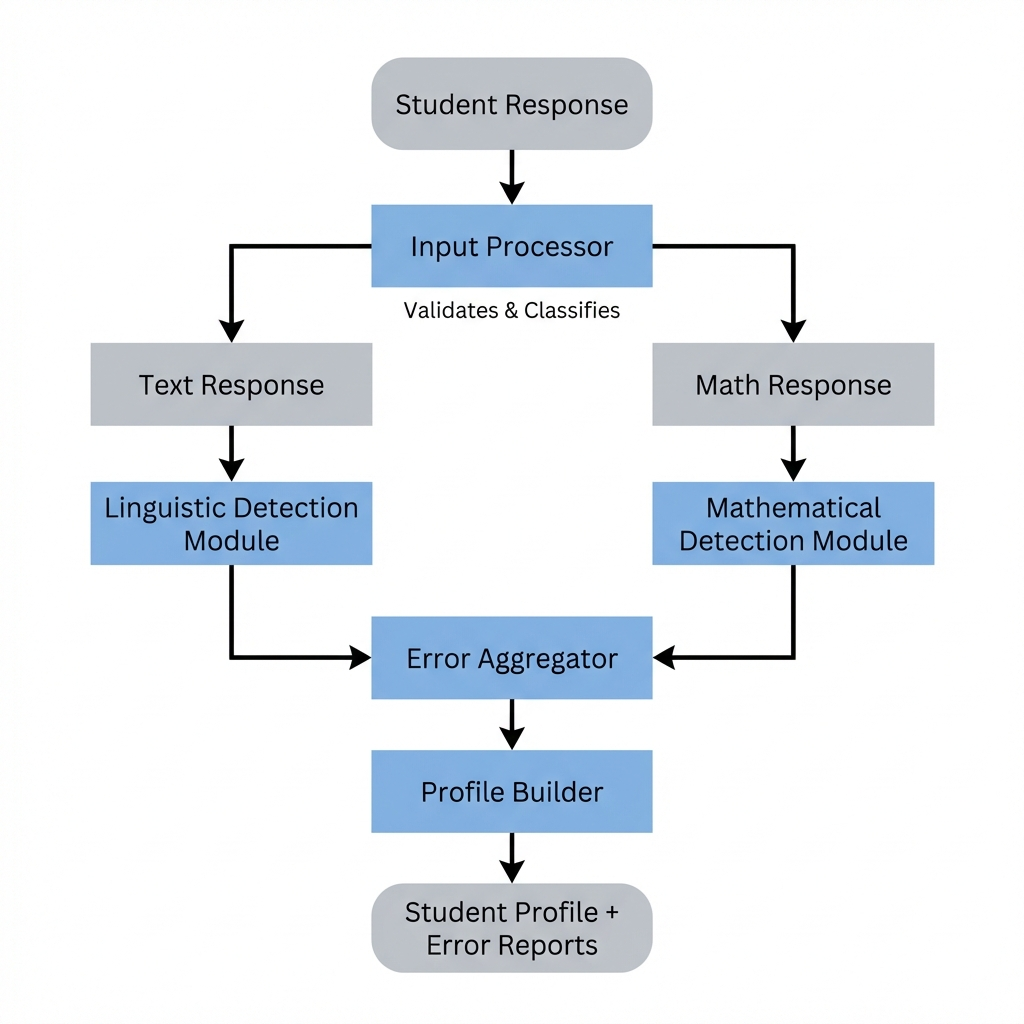
\includegraphics[width=0.85\textwidth]{figures/dataflow.png}
\caption{System data flow from student response to difficulty profile.}
\label{fig:dataflow}
\end{figure}

\subsection{Technology Stack}
\label{sec:impl_arch_stack}

The implementation uses Python (3.10--3.12), PyTorch and Hugging Face Transformers for the neural linguistic model, scikit-learn \parencite{Pedregosa2011} for the classical classifiers and clustering, and the ERRANT toolkit's M2 annotation format \parencite{BryantFeliceBriscoe2017} as the interchange format for real grammatical-error data. Phonetic matching uses the Metaphone algorithm \parencite{Philips1990} via the \texttt{jellyfish} library. Neural training was performed on a single consumer GPU (NVIDIA RTX 5070, 12\,GB VRAM); all other components run on CPU. All datasets, trained models, and experiment outputs are serialized as JSON or CSV for reproducibility.

\section{Linguistic Error Detection Module}
\label{sec:impl_ling}

The linguistic module identifies phonological (\texttt{PHONO}), orthographic (\texttt{ORTHO}), and segmentation (\texttt{SEG}) error spans in typed student text (taxonomy defined in Section~\ref{sec:method_tax_ling}), formulated as token-level sequence labeling with a BIO scheme over seven labels (\texttt{O} plus \texttt{B-}/\texttt{I-} variants of the three categories).

\subsection{Taxonomy Mapping Layer}
\label{sec:impl_ling_taxmap}

Public grammatical error correction (GEC) corpora annotate errors with ERRANT's generic type system (e.g., \texttt{R:SPELL}, \texttt{R:ORTH}), not with this thesis's difficulty-oriented categories. A deterministic mapping layer translates ERRANT-annotated edits into the thesis taxonomy:

\begin{itemize}
    \item An edit whose original and corrected strings contain the same letters grouped into a different number of space-separated tokens is mapped to segmentation (\texttt{ERR-SEG}), e.g., \emph{some times} $\rightarrow$ \emph{sometimes}. Edge punctuation is stripped before comparison, so sentence-boundary fixes (e.g., \emph{we} $\rightarrow$ \emph{. We}) are correctly excluded.
    \item \texttt{R:SPELL} edits are split into phonological and orthographic misspellings by phonetic faithfulness. If the misspelling and its correction share a Metaphone code, the misspelling preserves the word's sound (\texttt{ERR-PHONO}, e.g., \emph{wach} $\rightarrow$ \emph{watch}); otherwise it is treated as a visual/rule-memory slip (\texttt{ERR-ORTHO}).
    \item Homophone confusions between two correctly spelled words (\emph{their}/\emph{there}, \emph{to}/\emph{too}) are matched against a curated closed-class lexicon and mapped to \texttt{ERR-ORTHO}, following the taxonomy in Chapter~3.
    \item All other edits (grammar, word choice, punctuation) are out of scope and mapped to \texttt{OTHER}, leaving their tokens labeled \texttt{O}.
\end{itemize}

In practice, this mapping could not be designed reliably against toy examples alone. An earlier version used a blanket ``same Metaphone code $\Rightarrow$ homophone confusion'' rule for any single-token replacement; validating the mapper against roughly 65{,}000 real BEA-2019 gold edits \parencite{Bryant2019} revealed that Metaphone is coarse enough for unrelated content-word substitutions to collide by coincidence, and that capitalization edits and punctuation-driven sentence splits leaked into \texttt{ERR-SEG} under naive string checks. Three such precision bugs were found and fixed only because the mapper was audited against real corpus data.

\subsection{Data Pipeline}
\label{sec:impl_ling_data}

The linguistic module is trained and evaluated on three kinds of data prepared by a common pipeline. These are real corpora of learner writing, rule-based synthetic data, and a benchmark built to measure domain shift, and each is described below.

\subsubsection{Real data}

Two public GEC corpora are converted into BIO-tagged training sentences through the same M2-parsing and taxonomy-mapping pipeline:

\begin{itemize}
    \item BEA-2019 W\&I+LOCNESS \parencite{Bryant2019}: 2{,}584 sentences containing at least one in-scope error;
    \item CLC FCE v2.1 \parencite{YannakoudakisBriscoeMedlock2011}: 4{,}331 in-scope sentences from the train and dev splits, for a combined pool of 6{,}915 real sentences. The FCE test split (383 in-scope sentences) is excluded from training entirely and reserved as a held-out benchmark.
\end{itemize}

In a sentence containing multiple edits, only in-scope edits are tagged; tokens belonging to out-of-scope errors remain \texttt{O}. This is a deliberate, documented simplification: those tokens are still errorful in a general GEC sense, but outside the thesis's difficulty taxonomy.

\subsubsection{Synthetic data}

The synthetic generator applies rule-based corruptions (phonetically-faithful substitutions, orthographic slips, word splits and merges) to clean base sentences, emitting BIO tags for each injected error span by construction. The scale and diversity of the base sentences turned out to matter. An initial version used 20 hand-written template sentences; a model trained on it reached a perfect held-out score, and the score proved to reflect memorization of the templates (Section~\ref{sec:impl_lessons}). The generator now draws from a pool of approximately 600{,}000 clean English sentences filtered from a public Wikipedia sentence corpus (5--18 words, plain punctuation), from which 1{,}000{,}000 corrupted training examples are produced. With unique base sentences in held-out evaluation, synthetic performance becomes a legitimate measure of generalization over the corruption distribution.

\subsubsection{Domain-shift benchmark}

Both real corpora contain adult second-language (L2) learner writing, and neither comes from the thesis's target population, so an additional benchmark was built from the Holbrook corpus: transcribed writings of 19 secondary-school children with severe literacy difficulties, originally published by \textcite{Holbrook1964} and distributed in error-annotated electronic form by \textcite{Mitton1985}. Each annotated error is routed through the taxonomy mapper with one extra rule: if the child's written form is itself a real English word, the error is only in scope if it is a curated homophone confusion; otherwise it is treated as an out-of-scope (typically grammatical) error. This prevents inflection errors (\emph{go} for \emph{goes}) from leaking into the spelling-oriented categories. The result is 531 BIO-tagged sentences used exclusively for evaluation, never training.

\subsection{Model Selection}
\label{sec:impl_ling_modelsel}

Four encoder families were considered. BERT and RoBERTa \parencite{Devlin2019,Liu2019RoBERTa} are the established baselines for token classification; XLM-RoBERTa \parencite{Conneau2020} would keep the door open to multilingual deployment; DeBERTa-v3 \parencite{He2023DeBERTaV3} reports the strongest published results on NER-style token classification among models trainable on a single consumer GPU. DeBERTa-v3-base was selected on that evidence, with two consequences accepted knowingly: its disentangled-attention architecture proved numerically fragile under default fine-tuning settings (a real cost, documented below), and it is English-centric (multilinguality deferred with the language decision of Chapter~3). The \texttt{xsmall} variant of the same family is used for CPU-only pipeline smoke tests, so that the test path exercises the exact production code with a smaller checkpoint. Sequence-to-sequence GEC architectures were excluded at the framing stage (Chapter~3): they solve correction, a harder and different problem than span detection, at much higher training cost.

\subsection{Model and Training Procedure}
\label{sec:impl_ling_training}

The detector fine-tunes DeBERTa-v3-base \parencite{He2023DeBERTaV3} with a token-classification head over the seven BIO labels. Subword continuations inherit the \texttt{I-} variant of their word's tag, and special tokens are masked from the loss.

Training follows a three-stage curriculum inspired by GECToR \parencite{Omelianchuk2020GECToR}: stage 1 trains on synthetic data only; stage 2 continues fine-tuning the stage-1 checkpoint on real data only; stage 3 continues from the stage-2 checkpoint on the combined pool. The stages are therefore chained: the stage-2 model is a synthetic-pretrained model subsequently fine-tuned on real data, not a model trained on real data alone. Comparing the three stages on a fixed real evaluation split measures the marginal value of each stage. The direct test of hypothesis H2 also requires a real-only baseline (the same encoder fine-tuned on the real pool alone, with no synthetic stage, under the stage-2 training configuration), which is reported in Chapter~5 (Section~\ref{sec:eval_ling_scratch}). Per-stage epoch counts were revised twice as the datasets grew: initial counts (15 epochs per stage) were chosen for the early 2{,}000-sentence synthetic set; after the synthetic pool grew 500-fold, stages 1 and 3 were reduced to 2 epochs (more data warrants fewer passes for a comparable number of gradient updates, and 15 epochs over $10^6$ examples would cost hours for no expected benefit), and stage 2 was reduced from 15 to 8 when the real pool grew 2.7-fold with the FCE integration.

Class imbalance needed special handling. BIO tagging in this setting is extremely imbalanced: typically over 85\% of tokens are \texttt{O}. Plain cross-entropy lets the model collapse to always predicting \texttt{O} (observed empirically: precision, recall, and $F_1$ all exactly zero). Standard inverse-frequency class weighting overcorrected: with the sklearn ``balanced'' formula (weight ratios around $133\times$), the model collapsed to always predicting the highest-weighted rare class instead, and dampened variants swung back to the all-\texttt{O} collapse. The stable solution was focal loss \parencite{Lin2017Focal}:
\begin{equation}
    \mathcal{L}_{\text{focal}} = -\,\alpha_{y_i}\,(1 - p_{y_i})^{\gamma}\,\log p_{y_i},
\end{equation}
with $\gamma = 2$ and mild class-weight nudges $\alpha \in [0.5, 3.0]$. Because focal loss automatically down-weights tokens the model already classifies confidently (the abundant easy \texttt{O} tokens), the class weights no longer need to carry the entire burden of rebalancing, which removed the brittleness observed with weighted cross-entropy. One detail affects correctness. The common shortcut $p_t = e^{-\mathcal{L}_{CE}}$ is valid only for unweighted cross-entropy; with class weights applied it silently computes $p_t^{\alpha}$ instead. The value $p_t$ is therefore computed directly from \texttt{log\_softmax}.

DeBERTa-v3's disentangled attention also proved numerically fragile under the default fine-tuning configuration: with learning rate $5\times10^{-5}$ and no warmup, gradients became NaN within a few dozen steps. The final configuration uses learning rate $2\times10^{-5}$, warmup over the first 10\% of steps, and gradient clipping at norm 1.0. A second, subtler source of NaN corruption was that the checkpoint loads in half precision by default; training then proceeded in fp16 without loss scaling (since mixed-precision mode was never requested), a known recipe for overflow. The model is therefore explicitly loaded in fp32. Finally, a hard post-stage check counts NaN parameter tensors after every stage, so that a corrupted checkpoint fails loudly instead of silently producing zero-precision evaluations that masquerade as a data problem.

\section{Mathematical Error Detection Module}
\label{sec:impl_math}

The mathematical module detects procedural bugs (malrules) in multi-digit subtraction and common misconceptions in fraction arithmetic, using two deliberately contrasted methods: exact symbolic malrule simulation, and a feature-based machine-learning classifier. The comparison between them is itself one of the thesis's research questions (Q3).

\subsection{Symbolic Malrule Simulation}
\label{sec:impl_math_malrule}

Following the buggy-procedure tradition of \textcite{BrownBurton1978} and \textcite{VanLehn1990}, each modeled misconception is implemented as an executable function that computes the answer a student applying that malrule would produce:

\begin{itemize}
    \item \texttt{SFL} (smaller-from-larger): in each column, the smaller digit is subtracted from the larger, regardless of position;
    \item \texttt{BORROW\_ZERO}: borrowing from a zero column is handled incorrectly (the zero is treated as 10 without propagating the borrow);
    \item \texttt{BORROW\_NO\_DEC}: the borrow is taken but the lending column is never decremented;
    \item \texttt{FRAC\_ADD}: numerators and denominators are added independently ($\frac{a}{b} + \frac{c}{d} = \frac{a+c}{b+d}$), the whole-number-bias misconception;
    \item \texttt{FRAC\_COMPARE}: fractions are compared by comparing numerators and denominators as independent whole numbers.
\end{itemize}

Classification compares a student's answer against every malrule simulation for the problem at hand: an exact match identifies the misconception. This yields perfect precision on answers that exactly follow a modeled malrule. By construction, it also has zero tolerance to any deviation from that malrule, a limitation quantified in Chapter~5.

A non-obvious property surfaced during dataset generation: for two-digit subtraction with a single borrow, SFL and BORROW\_NO\_DEC are numerically identical; they only diverge at three or more digits. The dataset generator detects and filters such collision cases, since an example whose label is formally ambiguous is noise for any downstream learner. The general point is that malrule distinguishability depends on problem structure, so diagnostic item design (e.g., including 3-digit problems) is part of the detection method and not a separate concern.

\subsection{Feature-Based ML Classifier}
\label{sec:impl_math_ml}

The contrasting method is a gradient-boosted decision tree classifier over hand-built numeric features of the (problem, student answer) pair: digit-wise differences, borrow indicators, magnitude relations, and answer-structure features. The implementation uses scikit-learn's \texttt{HistGradientBoostingClassifier}; the histogram-based variant was adopted after the exact-boosting implementation failed to scale (it could not finish fitting 50{,}000 rows in the time the histogram version fits 700{,}000). Training data comes from the same malrule generator, with 1{,}000{,}000 examples per operation family; generation ranges (operand digit counts, fraction numerator/denominator bounds) were widened so that this many unique problems exist, the same uniqueness concern as in the linguistic synthetic data but in a milder form.

The two methods embody opposite trade-offs: the symbolic detector is exact, interpretable, and brittle, while the classifier is approximate and robust to perturbations. Chapter~5 measures this directly by evaluating both on malrule answers with and without superimposed digit-slip noise.

\section{Student Profiling Module}
\label{sec:impl_profile}

The profiling module aggregates per-response error labels into per-student feature vectors and clusters them into difficulty profiles. Because no public dataset provides longitudinal, per-student, error-labeled responses for this population (Chapter~3), evaluation combines a controlled simulation with two real-data grounding studies.

\subsection{Feature Representation}
\label{sec:impl_profile_features}

Each student is represented by the proportion of each error type among their errors (8 features spanning both modules' vocabularies), the overall error rate, and the temporal trend (slope of per-session error counts). The overall error rate is included explicitly because proportion-only features are mathematically blind to profiles that differ in error frequency but not in error mix. A low-difficulty student and a high-difficulty student with uniform error distributions have identical proportion vectors. This blindness was observed empirically (two such simulated archetypes were unrecoverable from proportions alone) before being fixed; it parallels the SFL/BORROW\_NO\_DEC collision in the math module, as both are information-theoretic limits of a representation, not code defects.

\subsection{Simulation Harness}
\label{sec:impl_profile_sim}

The simulator defines profile archetypes (e.g., phonologically-dominant, fraction-dominant, low-difficulty), samples multi-session response histories biased toward each archetype's error distribution, and measures whether unsupervised clustering (KMeans and HDBSCAN \parencite{Campello2013HDBSCAN}) recovers the known ground truth, scored by Adjusted Rand Index \parencite{HubertArabie1985}. It also serves a two-factor experiment (archetype separability $\times$ observations per student) whose results (Chapter~5) quantify how much data a real deployment must collect before profiles become trustworthy.

\subsection{Real-Data Grounding}
\label{sec:impl_profile_real}

Two studies connect the simulation's assumptions to real data:

\begin{itemize}
    \item Real error-mix archetypes (Holbrook). The per-student error distributions extracted from the Holbrook corpus (19 children with literacy difficulties) are clustered in the module's own feature space, testing whether archetype-like structure (distinct dominant error types) exists in real struggling writers at all, beyond what the simulation assumes.
    \item Real longitudinal stability (ASSISTments). The ASSISTments 2009--10 skill-builder dataset \parencite{Feng2009Assistments} provides 525{,}534 real math responses from 4{,}217 students. Per-student behavioral features (accuracy, mean attempts, hint-request rate, median first-response time, repeated-failure rate) are clustered, and stability is tested by a split-half design: each student's history is split into odd- and even-indexed responses, features and clusters are recomputed independently on each half, and agreement between the two assignments is measured by ARI. High agreement indicates that profiles are stable per-student traits and not session noise, which is the empirical precondition for difficulty profiling to be meaningful (H3).
\end{itemize}

\section{Pilot Prototype and Case Study}
\label{sec:impl_prototype}

To connect the modules to their intended use, a small web prototype wraps the trained system end-to-end: a student view serves rounds of one writing task (answered in English) plus subtraction and fraction problems generated with the same constraints as the training generator; a teacher dashboard aggregates each student's detected errors into the profiling module's feature representation, showing error-type proportions, the dominant pattern, and whether it persists across sessions. Storage is a local SQLite file by design (no accounts, no network), the appropriate privacy posture for a future school pilot, and the dashboard is framed strictly as formative (``error patterns''), never diagnostic.

The prototype is deliberately thin (a single Flask module), but building it surfaced two deployment findings that pure benchmark evaluation had not:
\begin{itemize}
    \item Raw argmax predictions are too eager for teacher-facing use. With real-data precision around 0.61 (Chapter~5), the model regularly flagged spans in error-free sentences. In an informal check on the prototype's smoke-test sentences (not a formal evaluation), a confidence threshold on the span prediction (default $0.55$, tunable per deployment) removed the false positives on error-free sentences while retaining the true detections on errorful ones. This threshold is the deployment-facing knob for the precision-recall trade-off that a single $F_1$ number hides.
    \item Preprocessing must match the training distribution exactly. An early version stripped sentence-final punctuation before inference; the model, trained on corpus-tokenized text where punctuation is always a token, systematically hallucinated segmentation errors on the final word of unpunctuated sentences. Punctuation-aware tokenization eliminated the artifact. In general, a detector's contract includes its tokenization, and violating it produces errors that look semantic but are purely mechanical.
\end{itemize}

\subsection{Screening Mode}
\label{sec:impl_prototype_screening}

The prototype's screening mode implements the closed-world regime of Section~\ref{sec:method_models_screening}. An item bank provides three linguistic item families (12 irregular ``orthographic-trap'' words, 12 short fully-decodable words, 10 compounds/multiword expressions) plus arithmetic items generated under the distinguishability policy (five-digit subtractions with a forced borrow-through-zero, admitted only when all three malrules yield pairwise-distinct answers, so any malrule-matching response identifies its misconception uniquely). The scorer aligns each written response with its known target and routes it through the audited taxonomy mapper (Section~\ref{sec:impl_ling_taxmap}); per-family error rates are compared against class norms, flagging deviations above $1.5$ standard deviations for teacher attention.

One routing rule differs deliberately from the free-text configuration: in free text, a misspelling that forms a real word (\emph{go} for \emph{goes}) is likely grammatical and is excluded; in dictation the target is fixed, so any deviation is a spelling attempt, including real-word outcomes (\emph{blent} for \emph{blend}, a true voicing error the free-text rule would wrongly discard). The scorer's self-test caught an error in this rule, so even ``deterministic'' components need the same validation discipline as learned ones.

\subsection{Portuguese Instantiation of the Screening Mode}
\label{sec:impl_prototype_screening_pt}

Chapter~3 argues that the screening regime, unlike the neural free-text path, is cheap to port across languages: it needs no corpus, no training and no encoder, only a language-specific item bank and a language-aware phonetic comparator. The claim was tested by building the European Portuguese (EP) instantiation, which required exactly two artifacts.

The first is a Portuguese phonetic comparator. The Metaphone role in the English pipeline (deciding whether a written form sounds the same as its target) is filled by a purpose-built EP grapheme-to-phoneme rule cascade (\texttt{screening/pt\_g2p.py}). The cascade covers the orthographic phenomena that generate Portuguese spelling traps: digraphs (ch, lh, nh, rr, ss), the silent h, context-dependent consonants (c and g before e/i, intervocalic s as /z/, ç, j, x), coda-nasal equivalence (\emph{campo}/\emph{canpo}), and EP word-final conventions (final -s/-z realized as the palatal fricative of European Portuguese, unstressed final o as /u/, elidable final e). Stress and vowel height are deliberately ignored: without a stress detector, accented and unaccented vowels map to the same segment, which routes accent omission (\emph{agua} for \emph{água}) through the sound-preserved path. This is the desired behavior, since accent omission is an orthographic-convention error. The comparator is explicitly not a general-purpose Portuguese G2P system; it is a closed-world instrument whose coverage claim extends to the item bank and its documented trap patterns, each locked in by a unit test (36 minimal pairs: 24 sound-preserving trap spellings that must compare equal, 12 sound-altering slips that must not).

The second is a Portuguese item bank, which re-instantiates the same three diagnostic families with EP-specific traps. The orthographic-trap words are those whose conventional spelling is unrecoverable from sound alone (\emph{hoje}, \emph{chave}, \emph{girafa}, \emph{casa}, \emph{cabeça}, eliciting ``oje'', ``xave'', ``jirafa'', ``caza'' and ``cabessa''). The fully decodable words allow only a sound-altering slip (\emph{pato}, \emph{dedo}, \emph{prato}). The segmentation items are built around attested Portuguese classroom fusions (\emph{de repente}$\,\to\,$\emph{derrepente}, \emph{às vezes}$\,\to\,$\emph{asvezes}, \emph{com certeza}$\,\to\,$\emph{concerteza}). The segmentation test required one Portuguese-specific refinement with no English analogue: fusing two words correctly by sound forces letter changes that Portuguese orthography demands at the new word-internal position (\emph{de~repente} fused is spelled with $\langle$rr$\rangle$, because a single intervocalic $\langle$r$\rangle$ would denote a different sound, and \emph{com~certeza} fused takes coda-nasal spelling). The scorer's segmentation normal form therefore collapses exactly these forced alternations (rr/r, ss/s, coda m/n) before comparing word material, so a child's phonologically faithful fusion is recognized as a boundary error and not misclassified as a spelling one.

The mathematical items required no porting at all: the distinguishability policy is symbolic and language-independent. The full Portuguese decision path (CORRECT, boundary error, sound-preserved error, sound-altering error) passes a 20-case archetypal self-test covering every designed trap pattern, and the prototype exposes the Portuguese worksheet alongside the English one (\texttt{/rastreio/<nome>?lang=pt}). The port consumed two artifacts and no data, which is the measured content of the portability claim: for screening, the Portuguese gap is an engineering task and not a data problem; for free text, it remains the data problem Chapter~6 describes. Neither the English nor the Portuguese item bank has yet been administered to children, so the diagnostic value of the item families is argued from the taxonomy, not measured.

\subsection{Case Study: A Simulated Classroom Walkthrough}
\label{sec:impl_prototype_casestudy}

To demonstrate the full pipeline in its intended usage pattern, and to make the system's behavior concrete for a reader who will not run it, the prototype was exercised end-to-end in a constructed classroom scenario. Three simulated students, each embodying one difficulty archetype from the profiling module's design, completed the same Portuguese screening worksheet (seed-fixed, so the walkthrough is exactly reproducible): student~A writes every orthographic-trap word as its phonetically faithful form but is otherwise flawless; student~B spells decodable words with sound-altering slips (voicing swaps, cluster reductions) and applies the smaller-from-larger malrule in every subtraction; student~C fuses or splits every multiword item. These are constructed personas, not real children. The point is mechanism demonstration, not empirical validation, and the thesis claims accordingly.

\begin{table}[ht]
\centering
\caption[Case-study walkthrough: per-family error rates for the three constructed archetypes.]{Case-study walkthrough: per-family error rates produced by the Portuguese screening scorer for the three constructed archetypes (12 dictation items, 3 diagnostic subtractions). Each archetype loads exclusively on its own family, and the malrule answer is identified uniquely.}
\label{tab:impl_casestudy}
\small\setlength{\tabcolsep}{4pt}
\begin{tabular}{lcccl}
\toprule
\textbf{Archetype} & \textbf{ORTHO-trap} & \textbf{PHONO-transp.} & \textbf{SEG} & \textbf{Math label} \\
\midrule
A: orthographic memory & 1.00 & 0.00 & 0.00 & correct \\
B: phonological        & 0.00 & 1.00 & 0.00 & SFL (all 3 items) \\
C: segmentation        & 0.00 & 0.00 & 1.00 & correct \\
\bottomrule
\end{tabular}
\end{table}

The teacher dashboard renders this as three clearly separated profiles. For each student it shows the dominant family and the class-norm z-score flags (each archetype flagged on exactly its own family), and for student~B it shows the uniquely identified subtraction misconception; the borrow-through-zero items admit only pairwise-distinct malrule answers, so the three identical wrong answers resolve to \emph{smaller-from-larger} with no ambiguity. The walkthrough exercises every component the thesis built (item selection under the distinguishability policy, the Portuguese comparator, closed-world scoring, norm-referenced flagging, and the profiling aggregation) in a single reproducible scenario. A school pilot would extend this demonstration from constructed personas to consented real classrooms (Chapter~6).

\section{Implementation Lessons}
\label{sec:impl_lessons}

Three classes of problems consumed most of the engineering effort, and each is a reusable lesson for similar systems:

\begin{enumerate}
    \item Silent numerical failure modes dominate loud ones. Every NaN episode in neural training traced back to configurations that produced no error message: a checkpoint silently loaded in fp16 without loss scaling; a focal-loss shortcut that silently computed the wrong probability under class weights; a default learning rate unstable for this architecture. The mitigations that worked were cheap and structural: explicit dtype control, post-stage NaN parameter audits, and diagnostic printing of predicted-tag distributions during every evaluation (a model collapsing to one class is visible instantly in the distribution, but invisible in a single $F_1$ number).
    \item Evaluation design is as failure-prone as model design. Two separate incidents produced misleadingly extreme scores: a perfect stage-1 score caused by 20 template sentences shared between train and eval (memorization, fixed by the 600k-sentence base pool), and a near-perfect combined-stage score caused by an evaluation set numerically dominated by synthetic examples ($\sim$99\% synthetic), which says nothing about real-data performance. Both motivated the final protocol of Chapter~5: every claim about real performance is measured on all-real, held-out benchmarks.
    \item Label mappings must be validated against real corpora. The taxonomy mapper and the Holbrook conversion each contained plausible-looking rules that were simply wrong on real data (Metaphone collisions, edge-punctuation segmentation artifacts, real-word grammar errors leaking into spelling categories). Auditing mapped output against thousands of real gold edits was the only thing that caught these.
\end{enumerate}

\section{Summary}
\label{sec:impl_summary}

The implemented system has three components. The linguistic error detector (DeBERTa-v3-base, focal loss, three-stage synthetic-to-real curriculum) is trained on 1M synthetic sentences and a pool of 6{,}915 real BIO-tagged sentences (90\% for training, 10\% held out), with two all-real held-out benchmarks including a domain-shift set from the target population. The mathematical error detector implements five executable malrules alongside a gradient-boosted classifier trained on 1M generated examples per operation family. The profiling module combines a feature design, a simulator, and two real-data grounding studies (real archetype shapes, real longitudinal stability) that operationalize H3. The next chapter evaluates all three modules.
